\documentclass[
	a4paper,
	oneside,
	BCOR = 10mm,
	DIV = 12,
	12pt,
	headings = normal,
]{scrartcl}

%%% Length calculations
\usepackage{calc}
%%%

%%% Support for color
\usepackage{xcolor}
\definecolor{lightblue}{HTML}{03A9F4}
\definecolor{red}{HTML}{F44336}
%%%

%%% Including graphics
\usepackage{graphicx}
%%%

%%% Font selection
\usepackage{fontspec}

\setromanfont{STIX Two Text}[
	SmallCapsFeatures = {LetterSpace = 8},
]

\setsansfont{IBM Plex Sans}[
	Scale = MatchUppercase,
]

\setmonofont{IBM Plex Mono}[
	Scale = MatchUppercase,
]
%%%

%%% Math typesetting
\usepackage{amsmath}

\usepackage{unicode-math}
\setmathfont{STIX Two Math}
%%%

%%% List settings
\usepackage{enumitem}
\setlist[enumerate]{
	label*      = {\arabic*.},
	leftmargin  = *,
	labelindent = \parindent,
	topsep      = 1\baselineskip,
	parsep      = 0\baselineskip,
	itemsep     = 1\baselineskip,
}

\setlist[itemize]{
	label*      = {—},
	leftmargin  = *,
	labelindent = \parindent,
	topsep      = 1\baselineskip,
	parsep      = 0\baselineskip,
	itemsep     = 1\baselineskip,
}

\setlist[description]{
	font        = {\rmfamily\upshape\bfseries},
	topsep      = 1\baselineskip,
	parsep      = 0\baselineskip,
	itemsep     = 0\baselineskip,
}

%%%

%%% Structural elements typesetting
\setkomafont{pagenumber}{\rmfamily}
\setkomafont{disposition}{\rmfamily\bfseries}

% Sectioning
\RedeclareSectionCommand[
	beforeskip = -1\baselineskip,
	afterskip  = 1\baselineskip,
	font       = {\normalsize\bfseries\scshape},
]{section}

\RedeclareSectionCommand[
	beforeskip = -1\baselineskip,
	afterskip  = 1\baselineskip,
	font       = {\normalsize\bfseries\itshape},
]{subsection}

\RedeclareSectionCommand[
	beforeskip = -1\baselineskip,
	afterskip  = 1\baselineskip,
	font       = {\normalsize\bfseries},
]{subsubsection}

\RedeclareSectionCommand[
	beforeskip = -1\baselineskip,
	afterskip  = -0.5em,
	font       = {\normalsize\mdseries\scshape\addfontfeatures{Letters = {UppercaseSmallCaps}}},
]{paragraph}
%%%

%%% Typographic enhancements
\usepackage{microtype}
%%%

%%% Language-specific settings
\usepackage{polyglossia}
\setmainlanguage{ukrainian}
\setotherlanguages{english}
%%%

%%% Captions
\usepackage{caption}
\usepackage{subcaption}

%\DeclareCaptionLabelFormat{closing}{#2)}
%\captionsetup[subtable]{labelformat = closing}

%\captionsetup[subfigure]{labelformat = closing}

\captionsetup[table]{
	aboveskip = 0\baselineskip,
	belowskip = 0\baselineskip,
}

\captionsetup[figure]{
	aboveskip = 1\baselineskip,
	belowskip = 0\baselineskip,
}

\captionsetup[subfigure]{
	labelformat = simple,
	labelformat = brace,
}
%%%

%%% Table typesetting
\usepackage{booktabs}
\usepackage{longtable}

\usepackage{multirow}

\usepackage{array}
\newcolumntype{v}[1]{>{\raggedright\arraybackslash\hspace{0pt}}p{#1}}
\newcolumntype{b}[1]{>{\centering\arraybackslash\hspace{0pt}}p{#1}}
\newcolumntype{n}[1]{>{\raggedleft\arraybackslash\hspace{0pt}}p{#1}}
%%%

%%% Drawing with TikZ
% \usepackage{tikz}
% \usepackage{tikzscale}
% \usetikzlibrary{
% 	arrows.meta, % Stealth arrow tips
% 	positioning,
% 	shapes,
% 	trees,
% }

% \tikzset{> = stealth}
%%%

%%% PDF inclusion
\usepackage{pdfpages}
%%%

%%% Links and hyperreferences
\usepackage{hyperref}
\hypersetup{
	bookmarksnumbered = true,
	colorlinks      = false,
	linkbordercolor = red,
	urlbordercolor  = lightblue,
	pdfborderstyle  = {/S/U/W 1.5},
}
%%%

%%% Length adjustments
% Set baselineskip, default is 14.5 pt
\linespread{1.068966} % ~15.5 pt
\setlength{\emergencystretch}{1em}
\setlength{\parindent}{1.5em}
\newlength{\gridunitwidth}
\setlength{\gridunitwidth}{\textwidth / 12}
%%%

%%% Custom commands
\newcommand{\allcaps}[1]{{\addfontfeatures{LetterSpace = 8, Kerning = Off}#1}}
%%%

\begin{document}
	\begin{titlepage}
		\begin{center}
			Міністерство освіти і науки України\\
			Національний авіаційний університет\\
			Навчально-науковий інститут комп'ютерних інформаційних технологій\\
			Кафедра комп'ютеризованих систем управління

			\vspace{\fill}
				Лабораторна робота №1.4\\
				з дисципліни «Інженерія програмного забезпечення»\\
				на тему «Створення графіку робіт та~ресурсів за~допомогою діаграми \textenglish{\allcaps{PERT}}»\\
				Варіант №3

			\vspace{\fill}

			\begin{flushright}
				Виконав:\\
				студент ННІКІТ\\
				групи СП-325\\
				Клокун В.\,Д.\\
				Перевірила:\\
				Голего Н.\,М.
			\end{flushright}

			Київ 2018
		\end{center}
	\end{titlepage}

	\section{Мета}
		Вивчити можливості перегляду інформації в~\textenglish{Microsoft Project}.

	\section{Завдання}
		Створити графік робіт за~допомогою діаграми~\textenglish{\allcaps{PERT}}, побудувати графік ресурсів, порівняти діаграми Ганта й~\textenglish{\allcaps{PERT}}.
		
	\section{Хід роботи}
		Створюємо графік робіт за допомогою діаграми \textenglish{\allcaps{PERT}}. Для цього відкриваємо файл проекту, переходимо в меню «Вид» та натискаємо на кнопку «Мережевий графік». Отримали графік робіт~(рис.~\ref{fig:01-network-diag})
		\begin{figure}[!htbp]
			\centering
			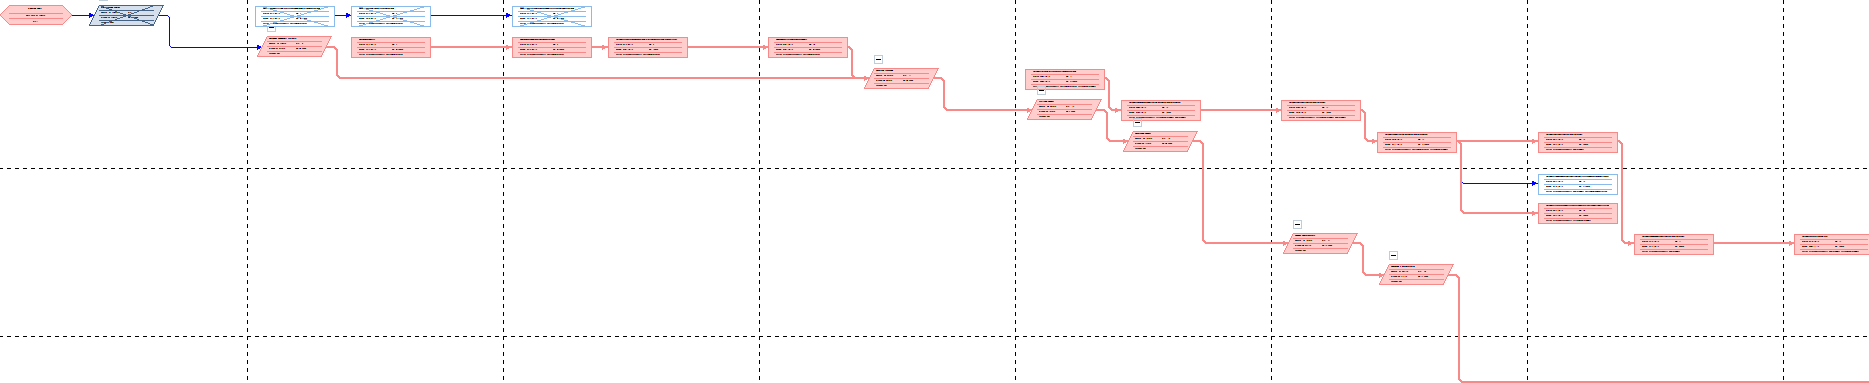
\includegraphics[height = 5\baselineskip]{./assets/y03s01-softeng-lab-04-p01-v02.png}
			\caption{Мережевий графік}
			\label{fig:01-network-diag}
		\end{figure}

		Складаємо діаграму в режимі використання робіт. Для цього у відкритому файлі проекту переходимо в меню «Вид» та натискаємо кнопку «Використання завдань». Отримали таблицю з режимом використання робіт~(рис.~\ref{fig:02-table-work-usage}).
		\begin{figure}[!htbp]
			\centering
			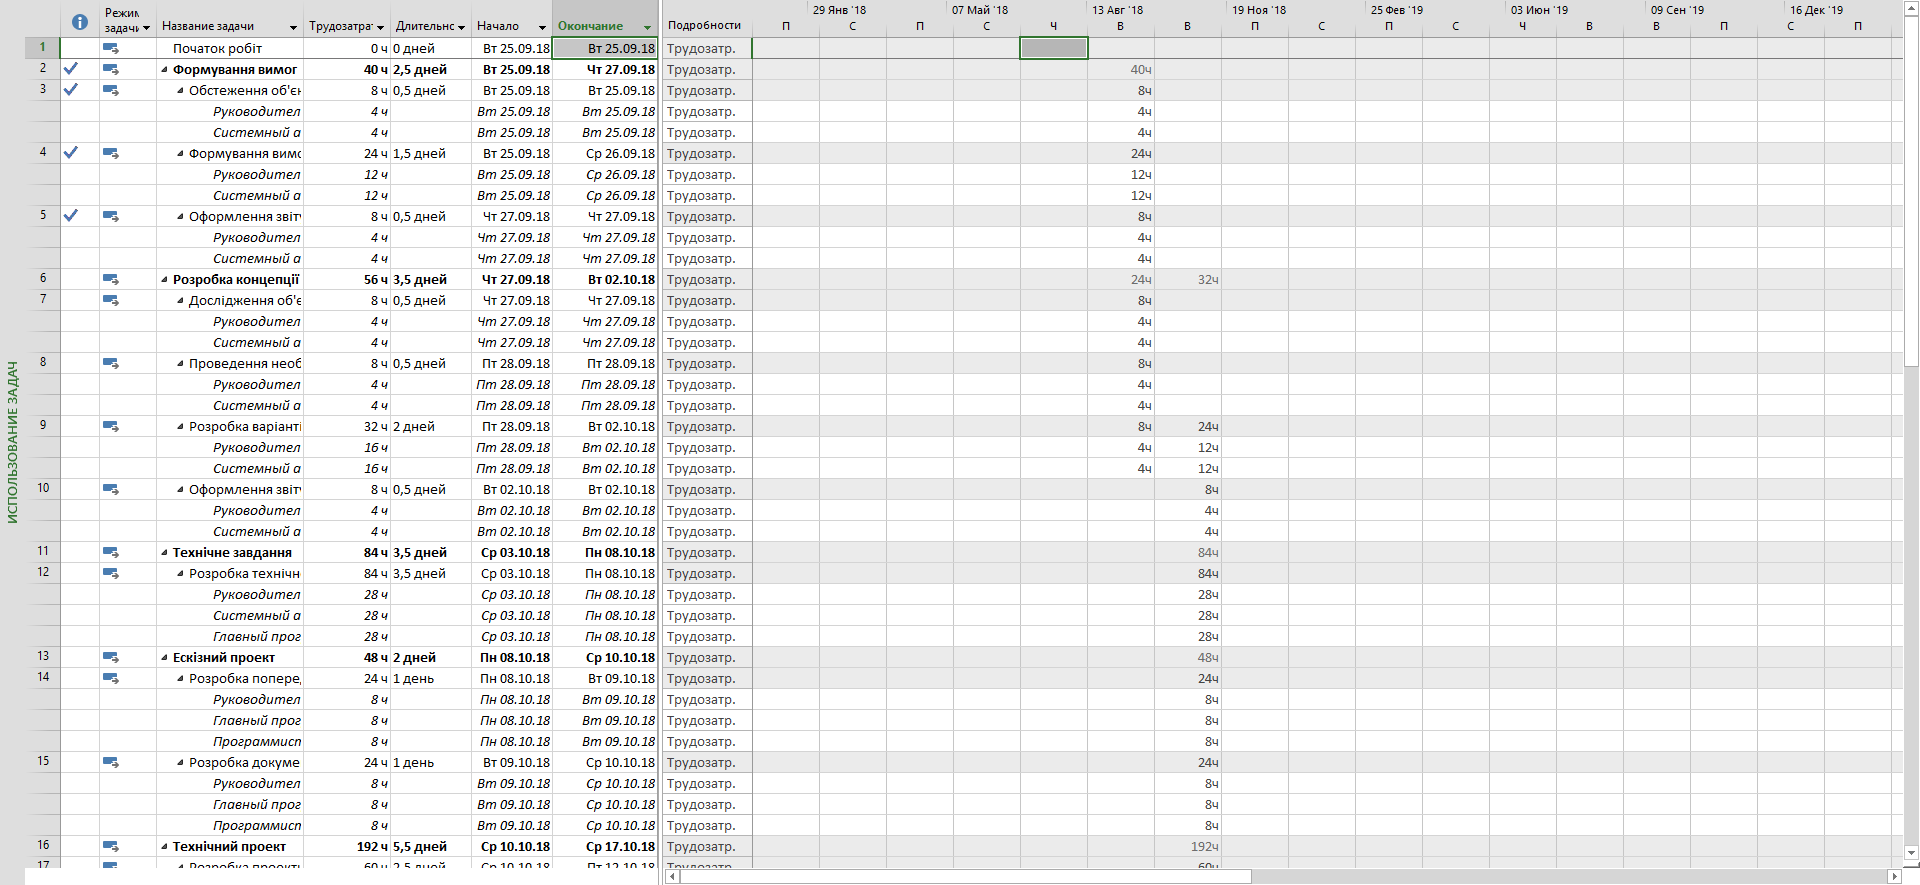
\includegraphics[height = 12\baselineskip]{./assets/y03s01-softeng-lab-04-p02-v02.png}
			\caption{Таблиця з режимом використання робіт}
			\label{fig:02-table-work-usage}
		\end{figure}

		Розглядаємо графік ресурсів. Графік ресурсів відображає інформацію про розподіл, обсяги робіт і вартості ресурсів. Для цього переходимо в меню «Вид», натискаємо кнопку «Інші представлення» та обираємо опцію «Графік ресурсів»~(рис.~\ref{fig:03-resource-schedule}).
		\begin{figure}[!htbp]
			\centering
			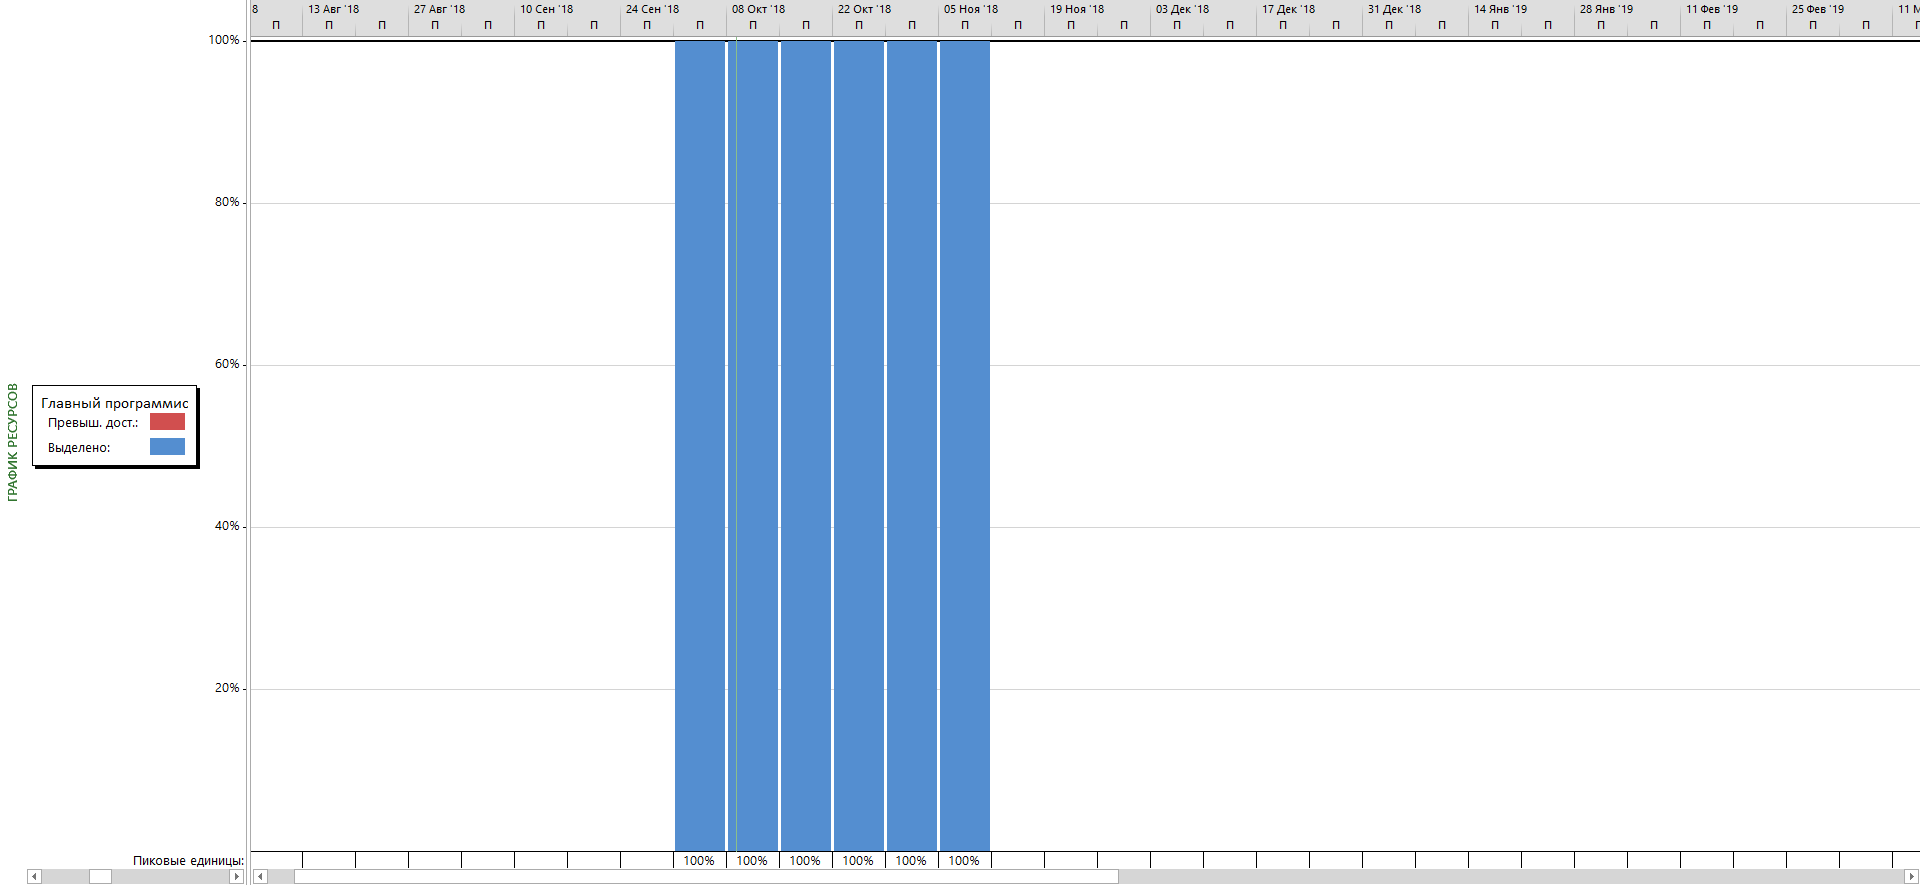
\includegraphics[height = 10\baselineskip]{./assets/y03s01-softeng-lab-04-p03-v02.png}
			\caption{Графік робіт ресурсу «Головний програміст»}
			\label{fig:03-resource-schedule}
		\end{figure}

		Розглядаємо використання ресурсів. Для цього переходимо в меню «Вид» і~натискаємо кнопку «Використання ресурсів»~(рис.~\ref{fig:04-resource-usage}).
		\begin{figure}[!htbp]
			\centering
			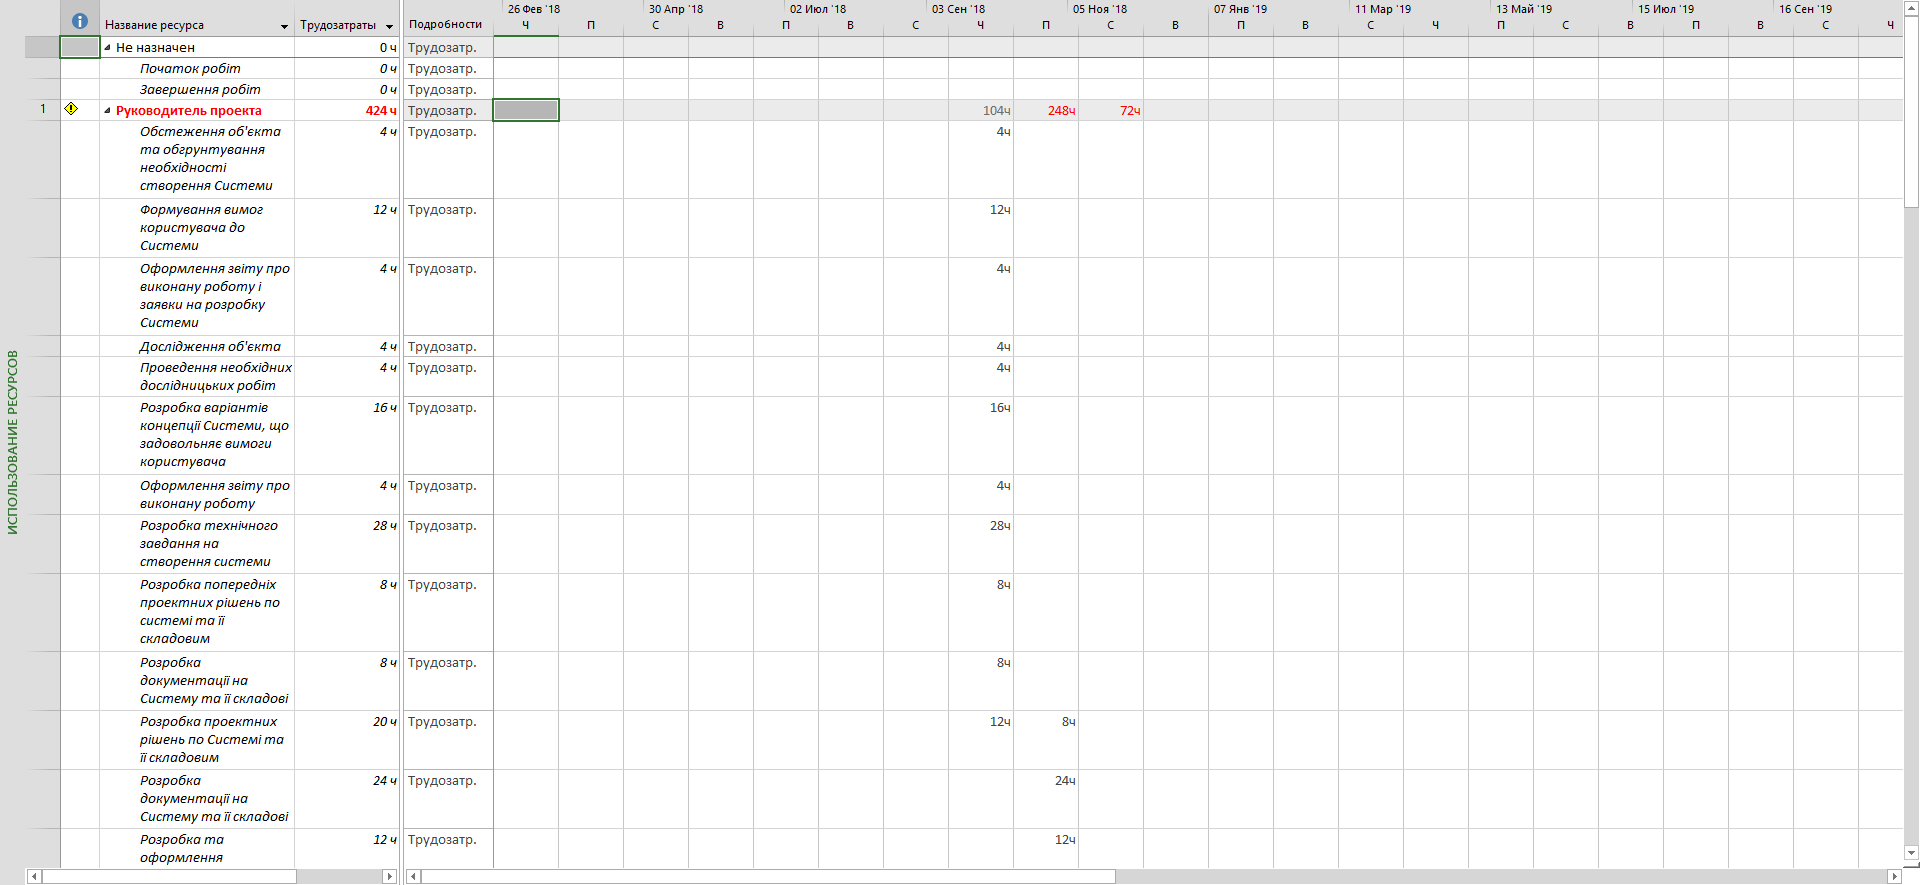
\includegraphics[height = 10\baselineskip]{./assets/y03s01-softeng-lab-04-p04-v02.png}
			\caption{Використання ресурсів}
			\label{fig:04-resource-usage}
		\end{figure}

	\section{Висновок}
		Під час виконання даної лабораторної роботи ми вивчили можливості перегляду інформації в~\textenglish{Microsoft Project}; створили графік робіт за~допомогою діаграми~\textenglish{\allcaps{PERT}}.

\end{document}
